% !TeX program = xelatex
% !TeX options = -shell-escape
% !TEX encoding = UTF-8

% --------------------------------------------------------------
% This is all preamble stuff that you don't have to worry about.
% Head down to where it says "Start here"
% --------------------------------------------------------------

\documentclass[12pt]{article}
\usepackage[margin=2cm]{geometry} % 頁面邊距設置
\usepackage{amsmath,amssymb,amsthm} % 數學相關套件
\usepackage{graphicx} % 圖形插入
\usepackage{booktabs} % 表格線條
\usepackage[AutoFakeBold,AutoFakeSlant]{xeCJK} % 中文支援
\usepackage{fancyhdr} % 頁首頁尾設置
\usepackage{xcolor,changepage,mdframed} % 顏色與框線相關
\usepackage{titlesec} % 標題格式
\usepackage{setspace} % 行距
\usepackage{minted} % 程式碼高亮（需安裝 Python 套件 pygments）
\usepackage{booktabs}
\usepackage{caption}
\usepackage{array}
\usepackage{ulem}
\usepackage[shortlabels]{enumitem} % 列表格式
\usepackage[colorlinks=true,linkcolor=black,urlcolor=blue,citecolor=blue]{hyperref}
% 超連結
\graphicspath{{images}}

% 字體設定 (xeCJK)
\setCJKmainfont{黑體-繁}
\setCJKmonofont{Noto Sans Mono CJK TC}

% 頁首/頁尾設定 (fancyhdr)
\pagestyle{fancy}
\fancyhead[L]{NASA Homework 10} % 可以用 \leftmark 取代
\fancyhead[R]{B13901011 吳亞倫}
\fancyfoot[C]{\thepage}
\renewcommand{\headrulewidth}{0.4pt}
\renewcommand{\footrulewidth}{0pt}
\setlength{\headheight}{15pt}

% tex-fmt: off
\newtheorem*{theorem}{Theorem}
\newenvironment{lemma}[2][Lemma]{\begin{trivlist}
\item[\hskip \labelsep {\bfseries #1}\hskip \labelsep {\bfseries #2.}]}{\end{trivlist}}
\newenvironment{exercise}[2][Exercise]{\begin{trivlist}
\item[\hskip \labelsep {\bfseries #1}\hskip \labelsep {\bfseries #2.}]}{\end{trivlist}}
\newenvironment{problem}[2][Problem]{\begin{trivlist}
\item[\hskip \labelsep {\bfseries #1}\hskip \labelsep {\bfseries #2}]}{\end{trivlist}}
\newenvironment{question}[2][Question]{\begin{trivlist}
\item[\hskip \labelsep {\bfseries #1}\hskip \labelsep {\bfseries #2.}]}{\end{trivlist}}
\newenvironment{corollary}[2][Corollary]{\begin{trivlist}
\item[\hskip \labelsep {\bfseries #1}\hskip \labelsep {\bfseries #2.}]}{\end{trivlist}}
\newenvironment{solution}{\begin{proof}[Solution]}{\end{proof}}
\newenvironment{answer}{\begin{proof}[Ans]}{\end{proof}}
\renewcommand\thesection{\Alph{section}.}      % 將 section 編號改成 A.、B.、C.…
\renewcommand\thesubsection{\Alph{section}.\arabic{subsection}.} % 將 subsection 編號改成 A.1、A.2、B.1…

% 樣式設定

\setminted{frame=lines, linenos, framesep=2mm, breaklines=true, breakanywhere=true, autogobble=true}

% 自訂框線環境
\newmdenv[
  linewidth=2pt, linecolor=gray, backgroundcolor=gray!10,
  topline=false, bottomline=false, rightline=false,
  skipabove=10pt, skipbelow=10pt, innerleftmargin=10pt,
  innerrightmargin=0pt, innertopmargin=5pt, innerbottommargin=5pt
]{myquote}

\newenvironment{mycolorbox}[1][gray]{
  \renewmdenv[
    linewidth=2pt, linecolor=#1, backgroundcolor=#1!10,
    topline=false, bottomline=false, rightline=false,
    skipabove=10pt, skipbelow=10pt, innerleftmargin=10pt,
    innerrightmargin=0pt, innertopmargin=5pt, innerbottommargin=5pt
  ]{myquote}
  \begin{myquote}
}{\end{myquote}}

\linespread{1.1}
% \usemintedstyle{xcode}
\AtBeginEnvironment{minted}{\vspace{-10pt}} % 可根據需求調整間距數值
\setminted{breaklines=true, breakanywhere=true, autogobble=true}

% tex-fmt: on
\begin{document}
\thispagestyle{fancy}

%------------------------------------------------------------
%                         Start here
% -----------------------------------------------------------

\begin{center}
  {\large \bfseries Network Administration / System Administration} \\
  \vspace{1em}
  {\Large \bfseries Homework 10} \\
\end{center}

\vspace{2em}

\begin{tabular}{@{}l l}
  \textbf{Student:} & 吳亞倫 \\
  \textbf{ID:} & B13901011  \\
  \textbf{Department:} & 電機工程學系
\end{tabular}
\bigskip

\begin{mycolorbox}[cyan]
  \textbf{Discussion Partners:}
  \begin{itemize}
    \item Classmates：賴泓安、鄭竣陽、喻慈恩
      \vspace{0.5em}
  \end{itemize}
\end{mycolorbox}

% Problem A
\section{Miscs}
\begin{mycolorbox}[teal]
  \textbf{Reference:}
  \footnotesize
  \begin{itemize}
    \item \href{https://note-on-clouds.blogspot.com/2018/11/wifi-bss-ess-ssid-essid-bssid.html}{WiFi 網路的識別: BSS, ESS, SSID, ESSID, BSSID}
    \item \href{https://community.ruijienetworks.com/forum.php?mod=viewthread&tid=5933}{What is difference among SSID, BSSID and ESSID?}
  \end{itemize}
\end{mycolorbox}

\begin{problem}{1.} 　
  \begin{itemize}
    \item SSID (Service Set Identifier) 是無線網路的「服務設定識別碼」，即你在裝置上看到、用來連線的網路名稱。它是一組長度最多 32 個字元的字串，用來區分不同的無線網路。同一個 SSID 下的裝置會在同一個 WLAN 中進行通訊。
    \item 而 BSSID (Basic Service Set Identifier) 是無線網路的「基本服務設定識別碼」，即用來分辨每一個 AP 的唯一識別碼。通常是 AP 的 MAC 位址。當有多個 AP 使用同一個 SSID 時，每個 AP 都會有不同的 BSSID，用來區分裝置現在是連到哪一個 AP。
    \item 一個 SSID 可以有多個 AP 來提供 WiFi 服務，因此會有多個 BSSID。使用者決定要連接哪一個 SSID 的 WiFi 之後，裝置之間會自動選擇最適合的 AP 來連接。這樣的架構可以讓使用者在不同的地點都能夠連接到同一個 SSID 的 WiFi，而不需要手動切換 AP。
  \end{itemize}
\end{problem}

\begin{problem}{2.} 　
  \begin{itemize}
    \item 同一個 AP 可以同時有很多 SSID，而同一個 SSID 也可以同時有很多 AP。
    \item 舉例來說，資工系上的 WiFi 具有兩個 SSID，分別是 \texttt{csie} 和\texttt{csie-5g}，提供了不同頻段的 WiFi 服務。這兩個 SSID 的 WiFi 都是由同一個 AP 提供的，並且可以同時存在於同一個 AP 上。同時，為了提供更好的無線網路覆蓋範圍，資工系的 WiFi 也會在不同區域設置多個 AP，每個 AP 都會有自己的 BSSID，但共用同一個 SSID。這樣的架構可以讓使用者在不同的地點都能夠連接到同一個 SSID 的 WiFi，而不需要手動切換 AP。
  \end{itemize}
  
\end{problem}

% Problem B
\clearpage
\section{HTML’s Wi-Fi Problem}
\begin{mycolorbox}[teal]
  \textbf{Reference:}
  \footnotesize
  \begin{itemize}
    \item \href{https://en.wikipedia.org/wiki/Friis_transmission_equation}{Friis transmission equation}
    \item \href{https://zh.wikipedia.org/wiki/%E5%88%86%E8%B2%9D}{分貝}
    \item \href{https://en.wikipedia.org/wiki/Signal-to-interference-plus-noise_ratio}{Signal-to-interference-plus-noise ratio}
  \end{itemize}
\end{mycolorbox}
\begin{problem}{1.}
  根據 Friis transmission equation，在 $P_t,\; G_t,\; G_r,\; d$ 皆相同的情況下，我們可以得知收到的訊號強度與波長平方成正比，即 $P_r \propto \lambda^2$。
  由於頻率與波長成反比，因此 2.4 GHz 的 Wi-Fi 頻率較 5 GHz 的 Wi-Fi 頻率波長長，故 2.4GHz 的 Wi-Fi 接收訊號強度較高。
\end{problem}
\begin{problem}{2.} 　
  \begin{itemize}
    \item 首先，將題目給的 $G_{t,db}$ 和 $G_{r,db}$ 換算回成線性增益 $G_t$ 和 $G_r$：
    \[
      G_t = 10^{\frac{G_{t,db}}{10}} = 10^{0} = 1, \quad G_r = 10^{\frac{G_{r,db}}{10}} = 10^{0} = 1
    \]
    \item 帶入 Friis transmission equation，其中 $c = 3\times10^{-8}$ m/s 為光速：
    \begin{align*}
      P_r/P_t &= G_t G_r \cdot \frac{\lambda^2}{(4\pi d)^2} = G_t G_r \cdot \frac{(\frac{c}{f})^2}{(4\pi d)^2} \\
      &= 1 \times 1 \times \frac{(3 \times 10^8)^2}{(4\pi \times 1 \times 5 \times 10^9)^2} \\ 
      &= 2.2797 \times 10^{-5} \\
      &= -46.42 \text{ dB}
    \end{align*}
  \end{itemize}
\end{problem}

\begin{problem}{3.} 　
  \begin{enumerate}[label=(\alph*)]
    \item 新 AP 設置前：
      \begin{itemize}
        \item 教授與 R103-front 之間的距離 $d_\text{front} = \sqrt{5^2 + 20^2} = \sqrt{425} \approx 20.62$ m 
        \item 教授與 R103-rear 之間的距離 $d_\text{rear} = \sqrt{25^2 + 10^2} = \sqrt{725} \approx 26.93$ m
        \item 由於教授距離 R103-front 較近，因此會優先連接 R103-front。視 Front 的強度為訊號強度 $S$，Rear 的強度為干擾強度 $I$。SINR 根據定義為 $S/I$，帶入公式如下：
        \[
          \text{SINR} = P_{r, \text{front}} / P_{r, \text{rear}} = (\frac{d_\text{rear}}{d_\text{front}})^2 = (\frac{725}{425}) \approx 1.71 \approx 2.3 \text{ dB}
        \]
      \end{itemize}
    \item 新 AP 設置後：
      \begin{itemize}
        \item 教授新的 AP 的距離為 $d_\text{new} = 5$ m
        \item 教授距離新 AP 的距離 $d_\text{new}$ 較近，因此會優先連接新 AP。因此視新 AP 的強度為訊號強度 $S$，R103-front 和 R103-rear 的強度和為干擾強度 $I$。因此，SINR 為：
        \[
          \text{SINR} = P_{r, \text{new}} / (P_{r, \text{front}} + P_{r, \text{rear}}) = (\frac{d_\text{new}^{-2}}{d_\text{front}^{-2} + d_\text{rear}^{-2}}) = \frac{1/25}{1/425 + 1/725} = 10.717 \approx 10.3 dB
        \]
      \end{itemize}
      我們可以發現增加新的 AP 之後， SINR 從約 2.3 dB 提升到約 10.3 dB，
      的確可以有效的提升教授的 Wi-Fi 連線品質。
  \end{enumerate}
\end{problem}

% Problem C
\section{Tiaosu’s Hotspot}
\begin{mycolorbox}[teal]
  \textbf{Reference:}
  \footnotesize
  \begin{itemize}
    \item \href{https://wiki.archlinux.org/title/Software_access_point#Wi-Fi_link_layer}{Arch Wiki: Software access point}
    \item \url{https://moda.gov.tw/press/multimedia/blog/11728}
    \item \href{https://www.cisco.com/c/dam/global/zh_tw/assets/docs/news2_1.pdf}{從加密技術看無線網路安全}
    \item \href{https://then.tw/aircrack-ng-wep/}{Aircrack-ng 破解 WEP 加密 Wi-Fi 密碼}
    \item \href{https://kysonlok.gitbook.io/blog/wireless/4_way_handshake}{WiFi 四次握手分析}
    \item \href{https://nordvpn.com/zh-tw/blog/deauthentication-attack/}{What is a deauthentication attack, and how does it work?}
    \item \href{https://www.cloudflare.com/zh-tw/learning/security/what-is-a-krack-attack/}{什麼是 KRACK 攻擊？| 如何防禦 KRACK 攻擊}
  \end{itemize}
\end{mycolorbox}

% Problem C.1
\subsection{Gimme expensive French meal}
\begin{problem}{1. }　
  \begin{itemize}
    \item 我假設 WiFi 的 interface 是 wlan0，橋接的 interface 是 br0。
    \item 我選擇使用 channel 6，即 2437 MHz 的頻道，因為這是最常用的頻道之一，且滿足中華民國 2.4 - 2.4835 GHz 的頻道規範。
    \item 我的設定檔案如下：
    \begin{minted}{bash}
      # /etc/hostapd/hostapd.conf

      interface=wlan0
      driver=nl80211
      bridge=br0

      ssid=tiaosu
      hw_mode=g
      channel=6
      country_code=TW

      macaddr_acl=0
      auth_algs=2
      wpa=3
      wep_key0=xxxxxxxxx
      wep_tx_keyidx=0
    \end{minted}
  \end{itemize}
\end{problem}

% Problem C.2
\subsection{WEP is dangerous!}
\begin{problem}{2. }　
  \begin{itemize}
    \item \textbf{Open System Authentication:} \\
          在此種方式當中，Client 會對先 AP 送出 Authentication Request。而 AP 在收到之後，都會回覆一個 Authentication Response。這個方式的認證過程是沒有任何的加密的，這意味著任何人都可以連接到 AP 上。
    \item \textbf{Shared Key Authentication:} \\
          在此種方式當中，會透過一個稱之為 challenge 的隨機字串來進行認證。首先，Client 會對 AP 送出 Authentication Request。AP 在收到之後，會回覆一個明文的 challenge 字串。接著，Client 會用事先共用的 WEP 金鑰加密該 challenge，並回傳給 AP。AP 會用相同金鑰解密，若解出來的明文與原始 challenge 相符，則回傳 Authentication Success，否則回傳失敗。相較於 Open System Authentication，這種方式的認證過程是有加密的，但仍然存在一些安全性問題。例如，共用金鑰洩漏的可能性極高。
  \end{itemize}
\end{problem}

\begin{problem}{3. }　
  \begin{enumerate}[label=(\alph*)]
    \item 第 11 筆封包看到 Client 對 AP 發送 Shared Key 的 Authentication Request，但是在第 13 筆封包中 AP 回覆 Responding STA does not support the specified authentication algorithm，這表示 AP 不支援 Shared Key 的認證方式，因此 Client 無法連接到 AP。

    而在後續 15 筆封包中，Client 對 AP 發送 Open System 的 Authentication Request，在第 17 當中 AP 回覆 Authentication Success，表示 Client 成功連接到 AP。
    \item 在這過程當中，攻擊者一般使用 ARP 協定，進行稱為 \texttt{ARP Replay Attack} 的攻擊方式。攻擊者會重複 replay 搜集到的 ARP 封包，並且將其發送到 AP 上。每次重播都會被 AP 重新加密並分配新的 IV，攻擊者便能快速蒐集到大量 IV，並且用來破解 WEP 金鑰。
    \item 在安裝完 aircrack-ng 之後，我們可以使用指令 \texttt{aircrack-ng WEPCapture.cap} 來破解 WEP 金鑰。
    執行完後出現以下的結果：
    \begin{minted}{bash}
      KEY FOUND! [ 63:73:6C:3C:33 ] (ASCII: csl<3 )
    \end{minted}
    \begin{figure}[H]
      \centering
      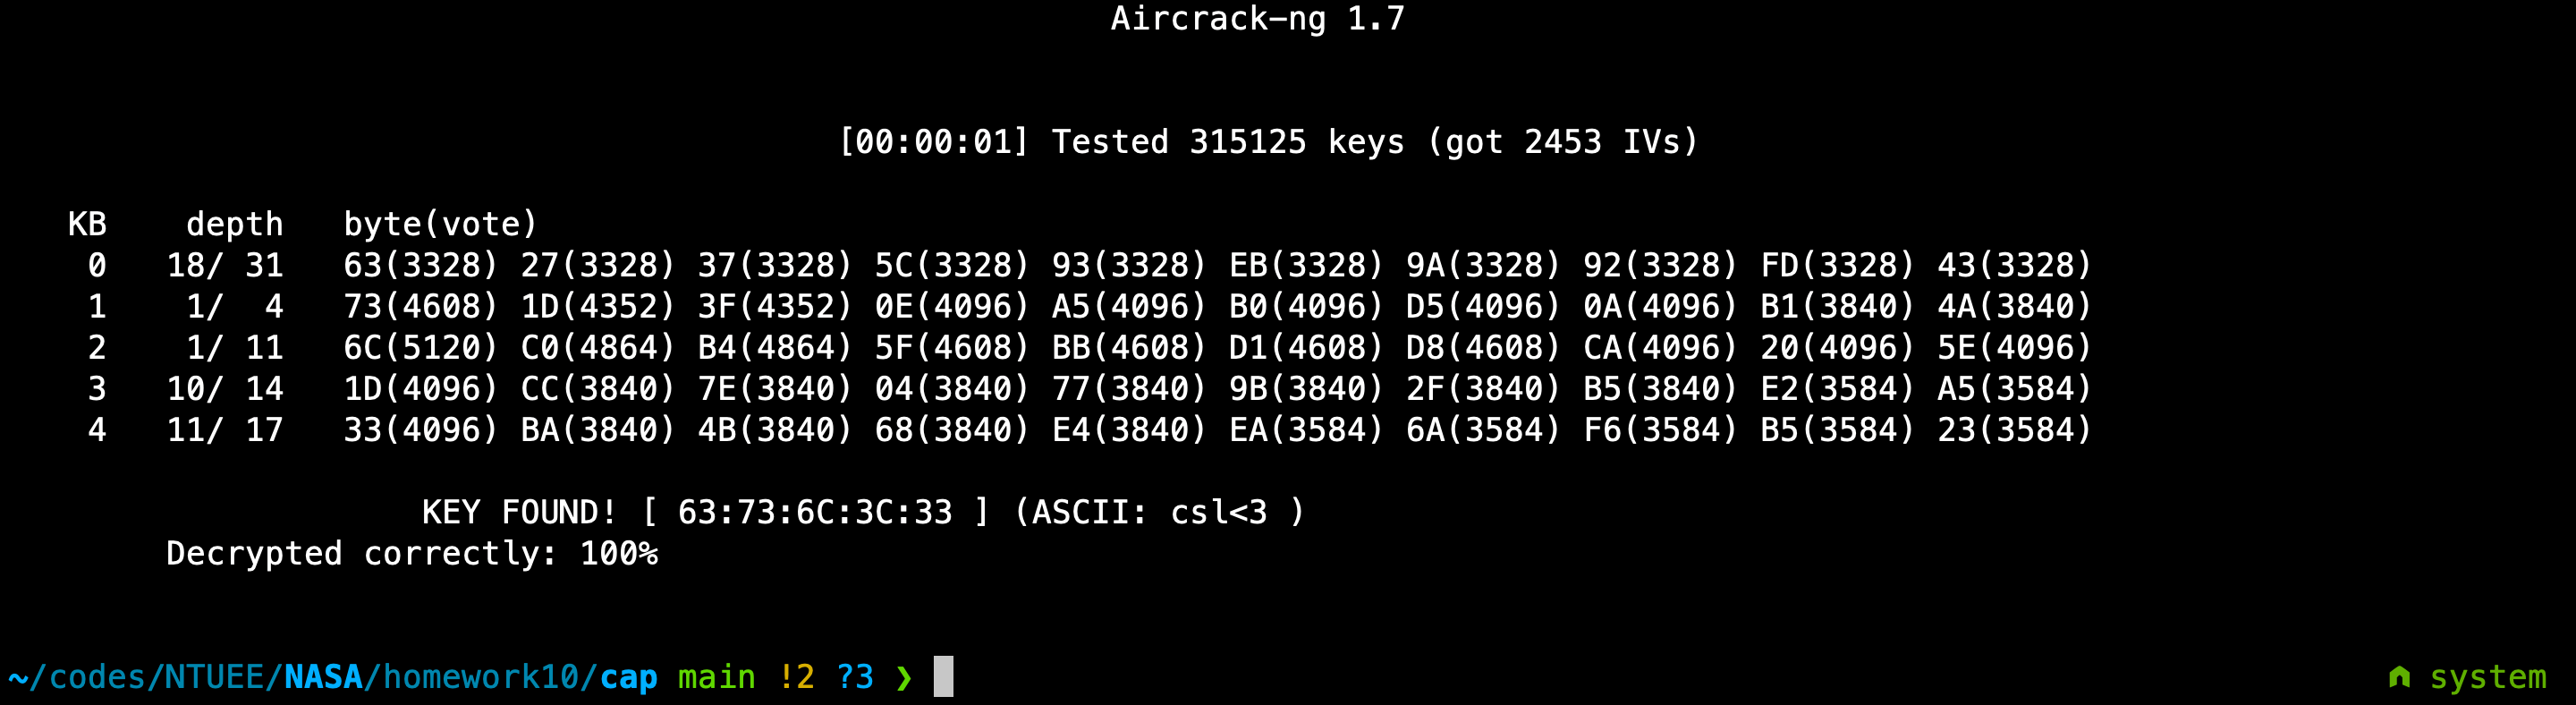
\includegraphics[width=0.6\textwidth]{c-3-c.png}
      \caption{Aircrack-ng 破解 WEP 金鑰}
      \label{fig:aircrack-ng}
    \end{figure}

    \item 進入 Preference > Protocols > IEEE 802.11 > Decryption Keys ，並且新增一個 key type 為 WEP，Key 為 63:73:6C:3C:33 的金鑰。解密後，可以在第 24276 筆封包看到 client 對 server (IP 和 Port 為\texttt{140.112.30.188:54321}) 發出請求，並且以 username: \texttt{tiaosu} 和 password: \texttt{ilovecsl} 登入。在第 24300 筆封包中，server 回覆 client 包含 flag 的回應，如下所示：
    \begin{minted}{text}
      Login successful! Although this is HTTP but WEP is so safe so I'll send the flag to you directly!!! NASA_HW10{W3P_15_N07_50_54F3}
    \end{minted}
  \end{enumerate}
\end{problem}

\begin{problem}{4. }
  WEP 的確很容易被破解並且截取當中的封包內容。然而，若網站是透過 https 加密的，則 WEP 封包被破解之後，依然有一層 TLS 的加密保護。這樣的話，攻擊者就無法直接看到封包內容，因為 TLS 會對傳輸的資料進行加密和驗證，即使攻擊者能夠截取到 WEP 封包，他們仍然需要破解 TLS 的加密才能獲取實際的資料內容。因此，WEP 雖然不安全，但如果網站使用 HTTPS 加密，則可以有效地保護資料的安全性。
\end{problem}

% Problem C.3
\subsection{I must get free hotspot}

\begin{problem}{5. }
    四次握手的核心目標是為了生成一個用來加密無線通訊的密鑰，並且確保雙方都擁有相同的密鑰。以下為我的四向交握循序圖：
  \begin{figure}[H]
    \centering
    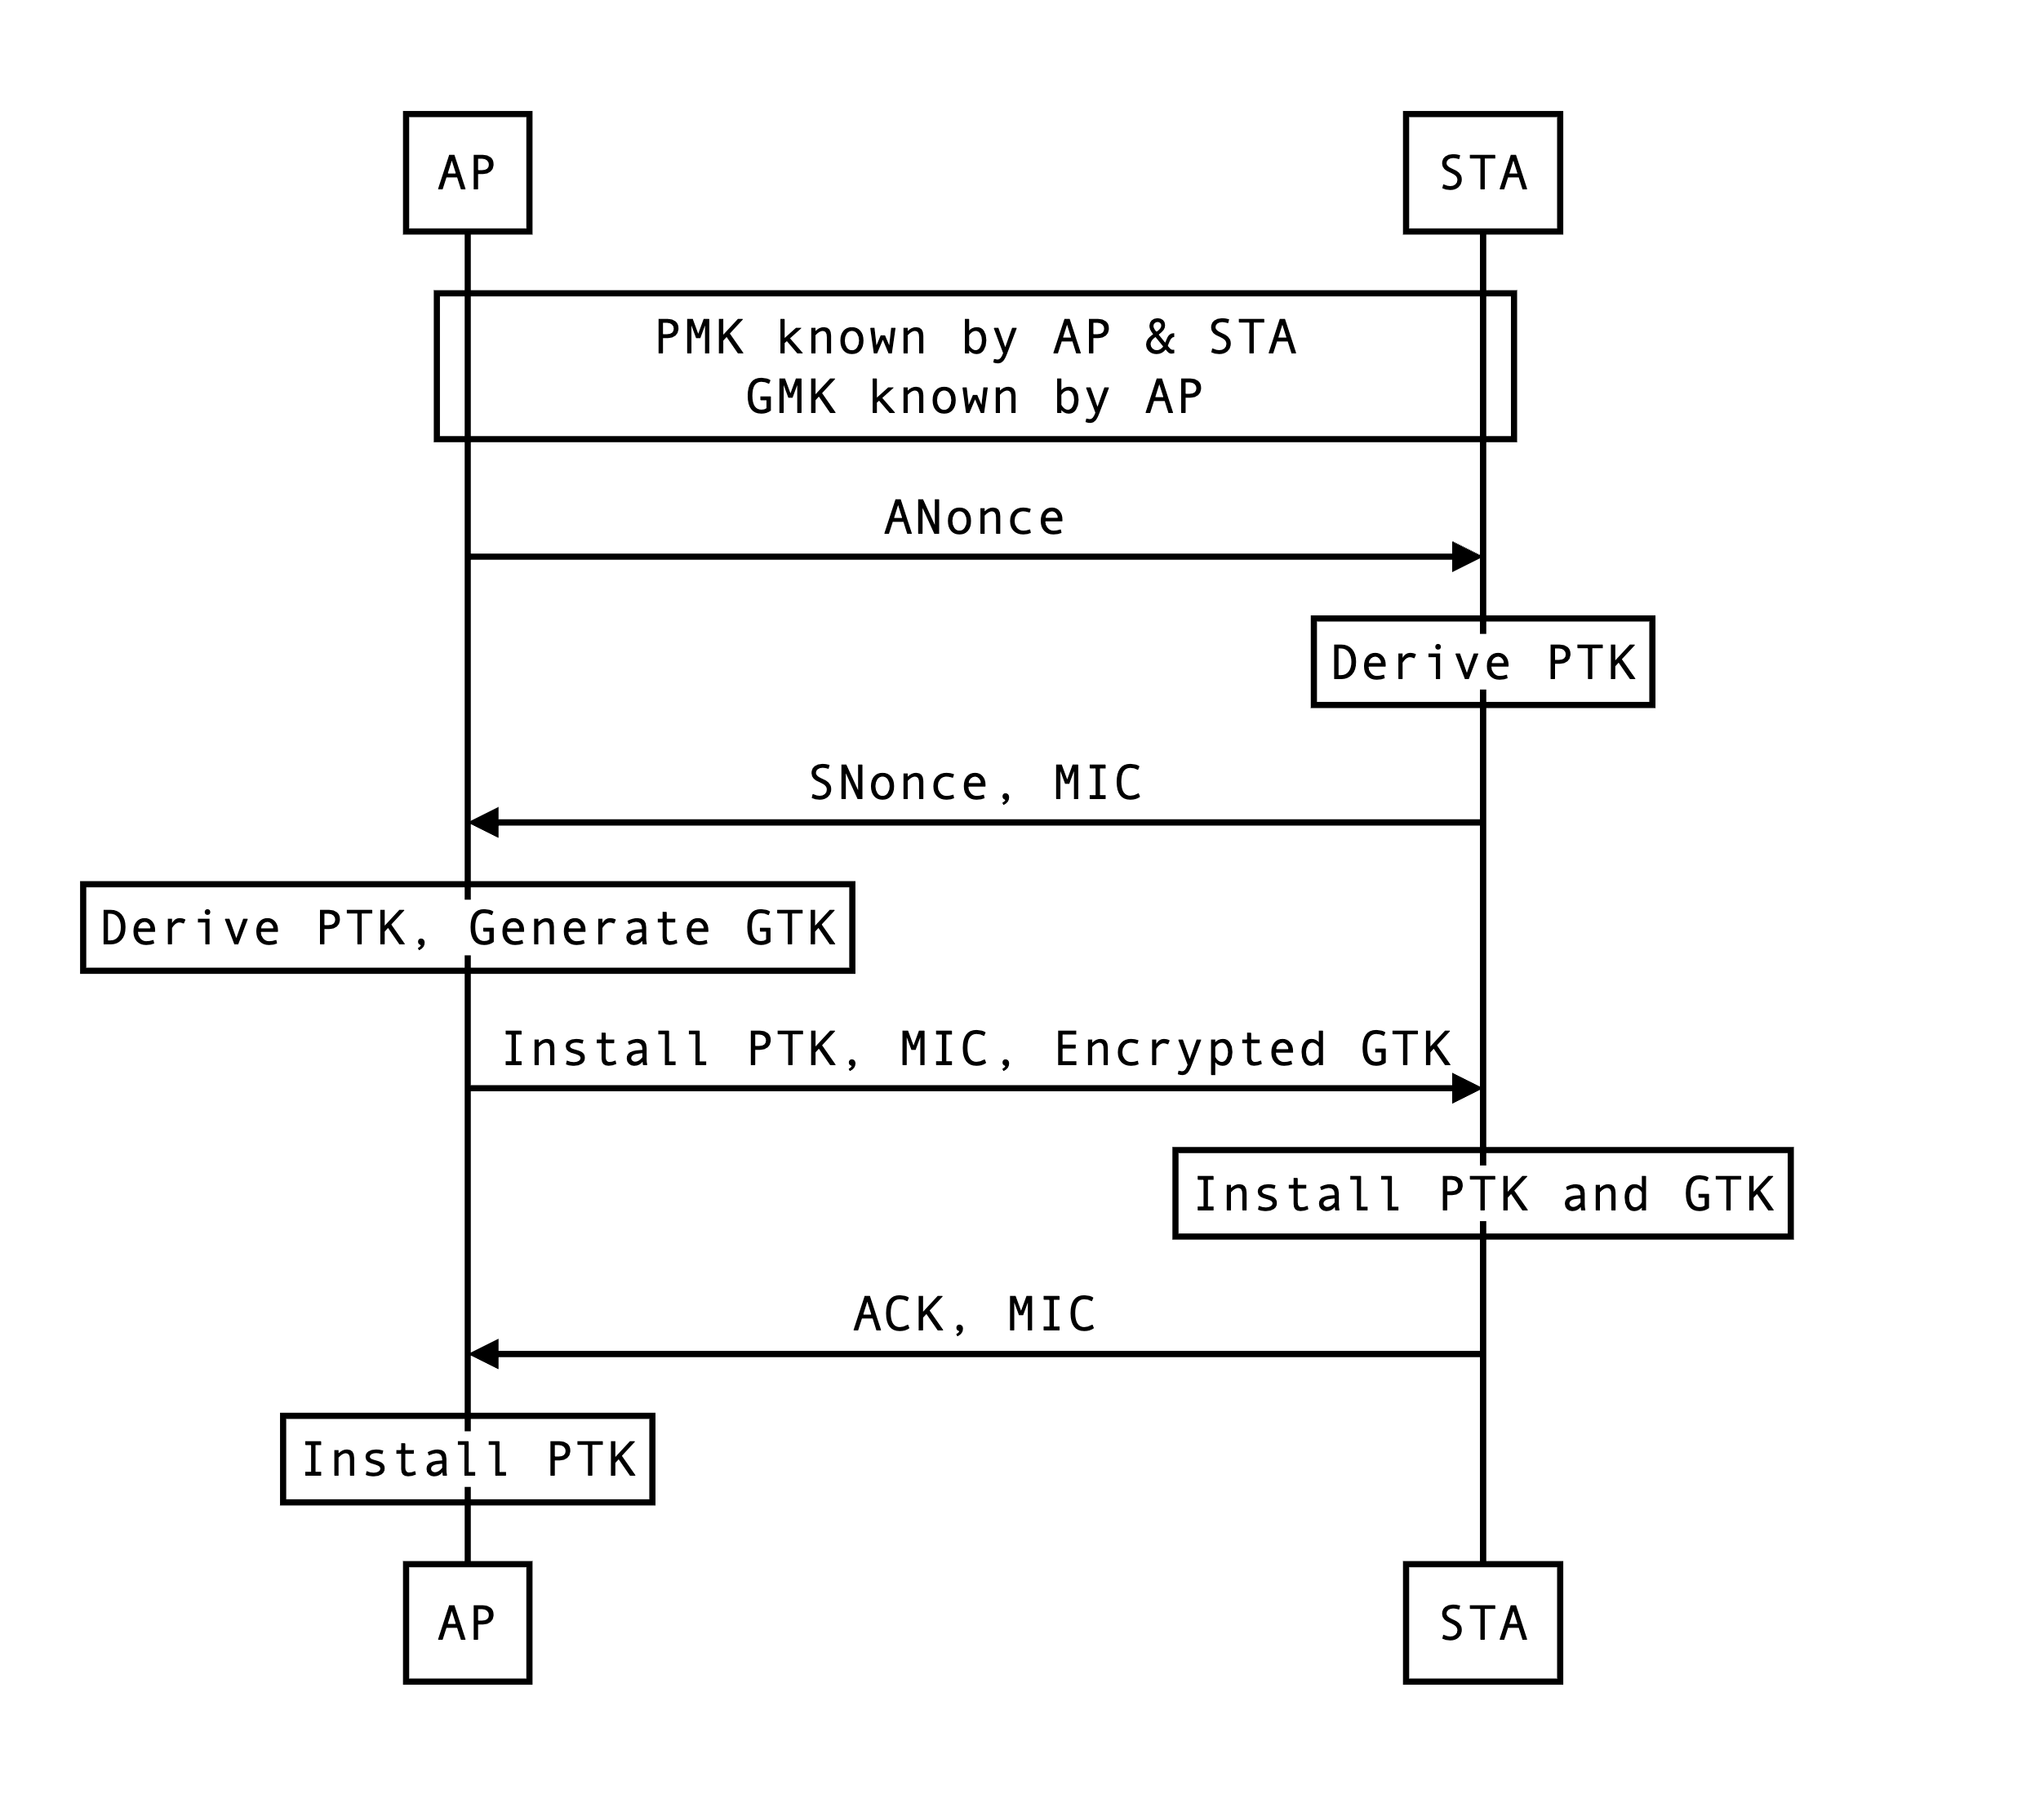
\includegraphics[width=0.75\textwidth]{c-5.png}
    \caption{四向交握循序圖}
    \label{fig:4-way-handshake}
  \end{figure}
\end{problem}

\begin{problem}{6. } Deauthentication Attack 是一種透過發送 Deauthentication 封包來斷開 Client 與 AP 之間的連線的攻擊方式，透過強迫 Client 重新連接到 AP，從而捕獲四次握手的封包。攻擊者就可以透過這些封包取得 ANonce、SNonce 和 MIC 等等資料，並且嘗試破解密碼。這種攻擊方式的原理是利用了 Wi-Fi 的設計缺陷，因為 Wi-Fi 協定並沒有對 Deauthentication 封包進行驗證，因此攻擊者可以輕易地偽造這些封包。
\end{problem}

\begin{problem}{7. }　
  \begin{enumerate}[label=(\alph*)]
    \item 根據封包內容，可以判斷 AP 的 MAC 位址為 \texttt{2C:CF:67:57:78:33}，而 Client 的 MAC 位址為 \texttt{BA:E0:E8:E8:4F:41}。
    \item 第一次握手的封包為第 21 筆封包。
    \begin{figure}[H]
      \centering
      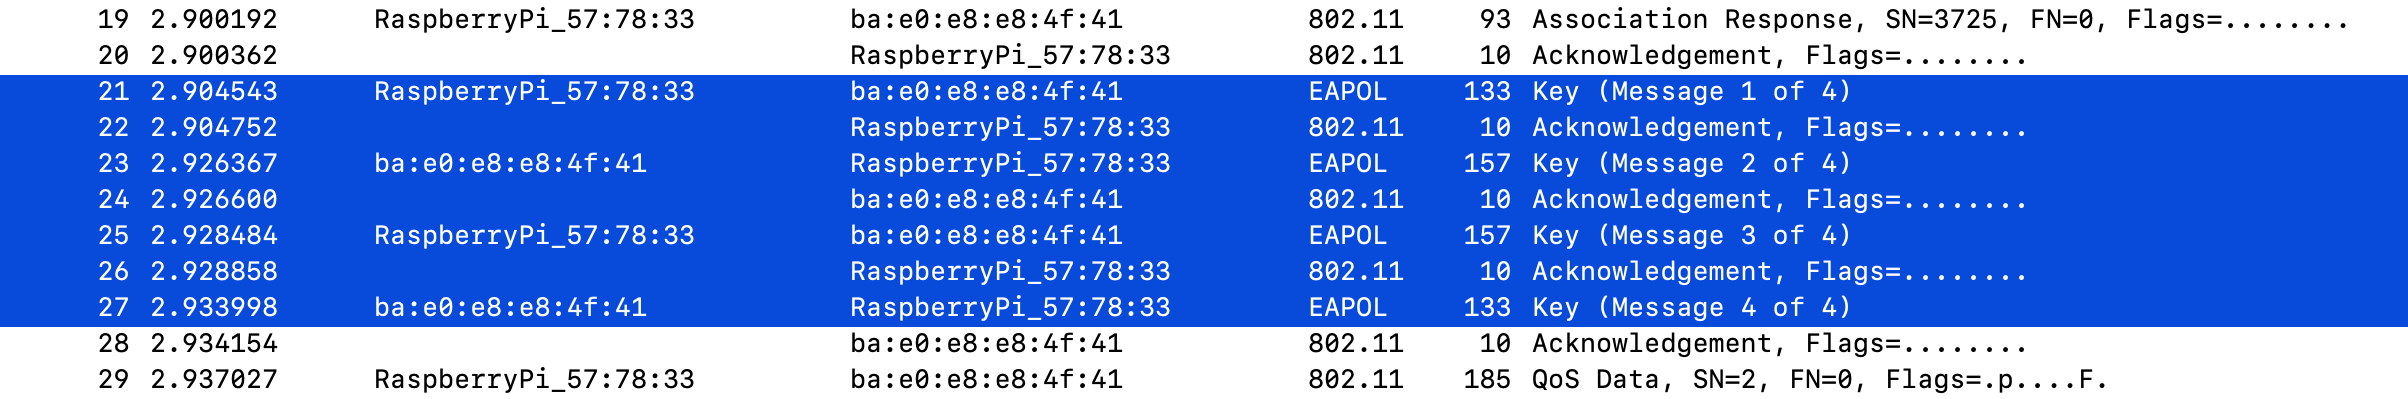
\includegraphics[width=0.9\textwidth]{c-7-b.png}
      \caption{第一次握手的封包}
      \label{fig:1st-handshake}
    \end{figure}
    \item 透過使用 \texttt{eapol} 作為過濾條件，可以找到四次完整的四次握手封包。
    \begin{figure}[H]
      \centering
      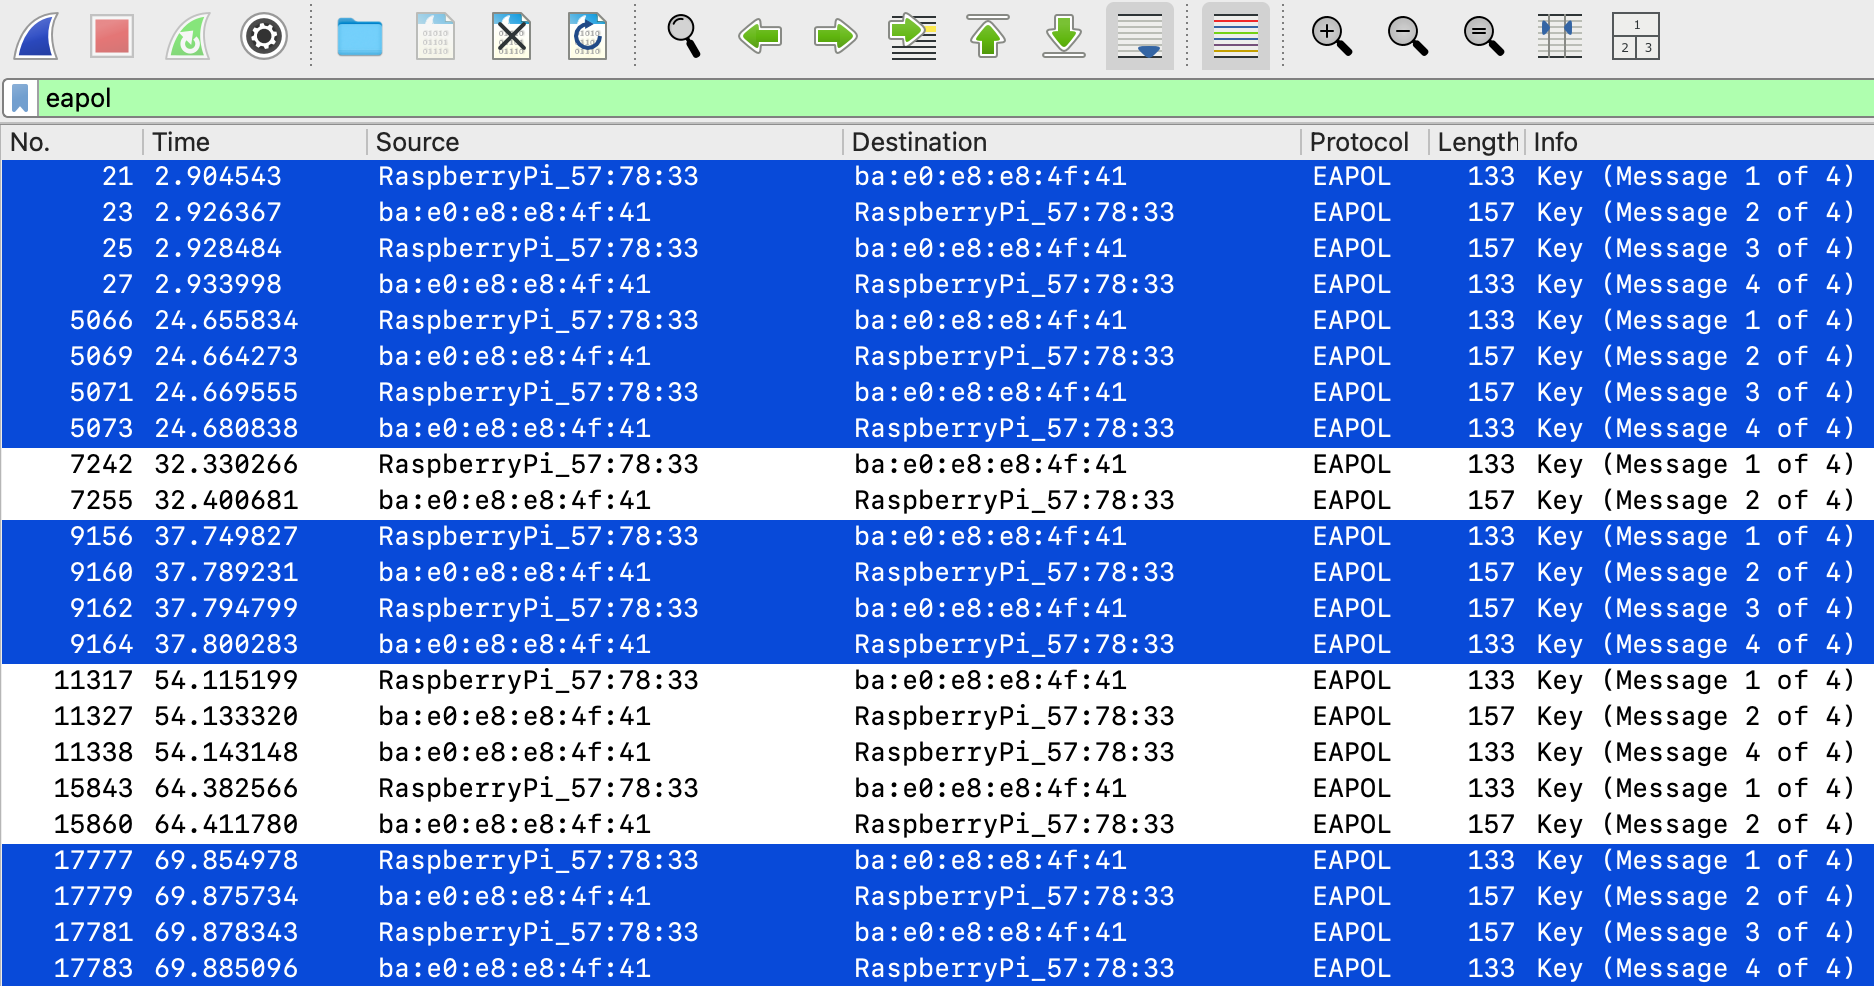
\includegraphics[width=0.7\textwidth]{c-7-c.png}
      \caption{四次握手的封包}
      \label{fig:4-way-handshake-packets}
    \end{figure}
    \item 我使用以下指令進行四次握手的解密，得到密碼為 \texttt{felwinter}。
    \begin{minted}{bash}
      aircrack-ng -w rocktiaosu.txt -b 2C:CF:67:57:78:33 DeAuthCapture.cap    
    \end{minted}
    \begin{figure}[H]
      \centering
      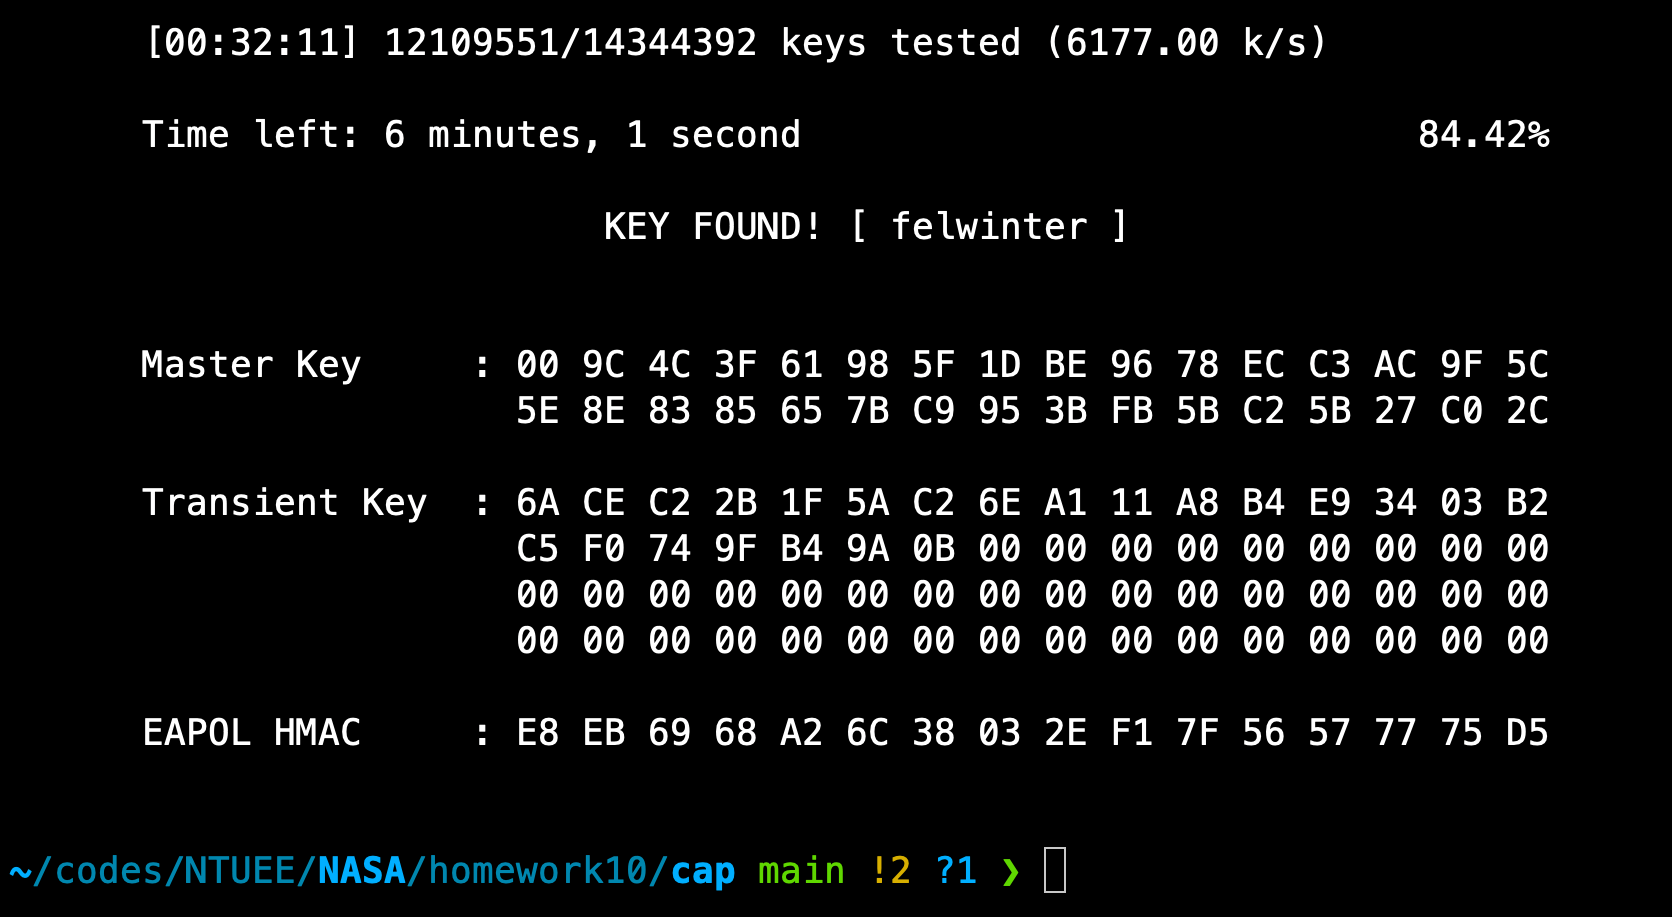
\includegraphics[width=0.7\textwidth]{c-7-d.png}
      \caption{破解 passphrase}
      \label{fig:crack-passphrase}
    \end{figure}
    \item 進到 Preferences > Protocols > IEEE 802.11 > Decryption Keys，新增一個 key type 為 WPA-PWD，Key 為 \texttt{felwinter} 的金鑰。解密後，可以在第 43 筆封包看到 DHCP ACK 的封包，給予 Client IP 位址為 \texttt{192.168.0.81}。
    \begin{figure}[H]
      \centering
      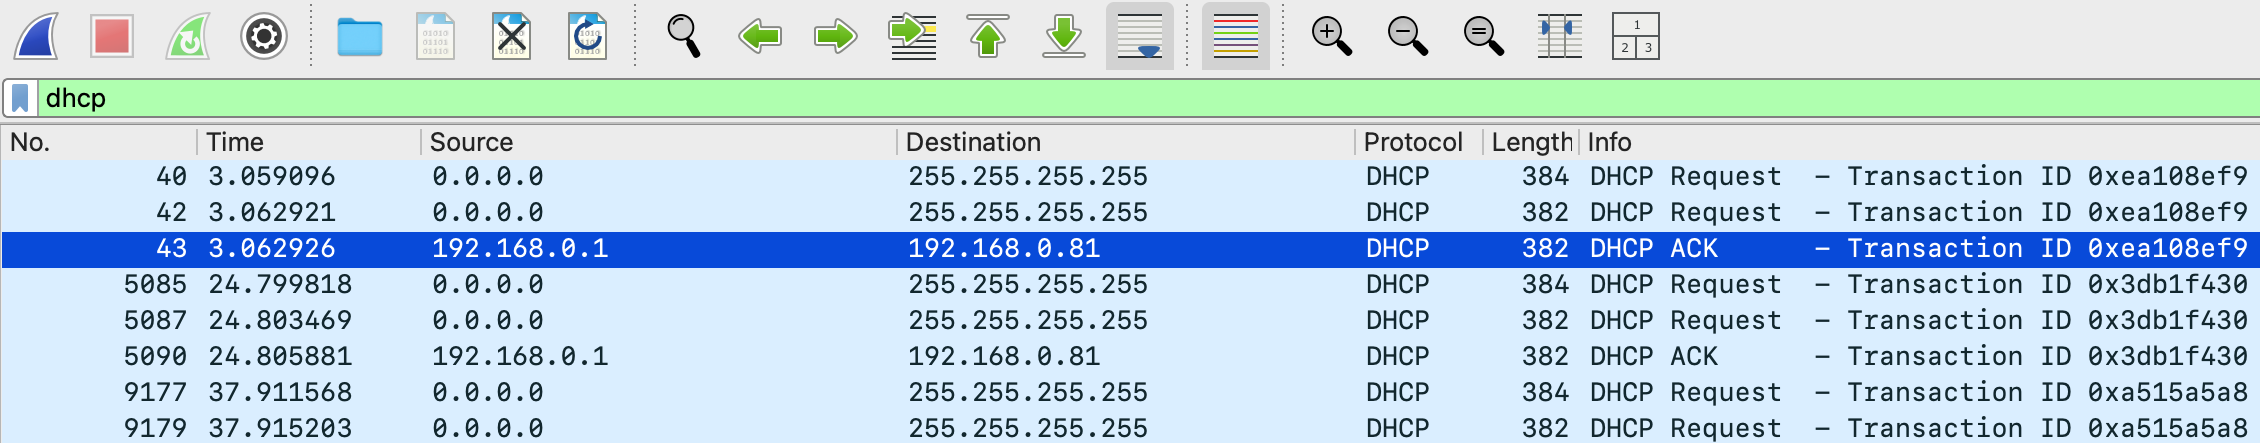
\includegraphics[width=0.9\textwidth]{c-7-e.png}
      \caption{DHCP ACK 的封包}
      \label{fig:dhcp-ack-packet}
    \end{figure}
  \end{enumerate}
\end{problem}

\begin{problem}{8. }KRACK attack 主要是用來針對 WPA2 的漏洞進行攻擊。為了更快地重新連線，Wi-Fi 在重連時只需要重新傳輸四次握手的第三部分。

攻擊者只要攔截並重放這個第三次握手封包，就能誘使客戶端重複安裝同一把 PTK 並重置內部的 Nonce，導致 keystream 重複使用。如此一來，攻擊者便可以利用已知的明文–密文對來解密後續封包，或偽造惡意封包，達到竊聽和中間人攻擊的目的。
\end{problem}

% -----------------------------------------------------------
%    You don't have to mess with anything below this line.
% -----------------------------------------------------------

\end{document}
